\documentclass[12pt,a4paper]{report}

% --- Paquets bàsics ---
\usepackage[catalan]{babel}
\usepackage[utf8]{inputenc}
\usepackage[T1]{fontenc}
\usepackage{lmodern}
\usepackage{geometry}
\usepackage{setspace}
\usepackage{graphicx}
\usepackage[hidelinks]{hyperref}
\usepackage{amsmath}
\usepackage{amsfonts}
\usepackage{amssymb}
\usepackage{float}
\usepackage{listings}
\usepackage{xcolor}

\lstdefinelanguage{CSharp}{
  language=[Sharp]C
}

\lstset{
  basicstyle=\ttfamily\footnotesize,
  breaklines=true,
  breakatwhitespace=false,
  postbreak=\mbox{\textcolor{red}{$\hookrightarrow$}\space},
  captionpos=b,
  frame=single,
  framerule=0.5pt,
  rulecolor=\color{gray!60},
  aboveskip=6pt,
  belowskip=6pt,
  keywordstyle=\color{blue},
  commentstyle=\color{gray},
  stringstyle=\color{teal},
  showstringspaces=false,
  tabsize=2
}
\begin{document}

\chapter{Teoria de Rapid SCADA}

\section{Introducció a Rapid SCADA}

\subsection{Què és Rapid SCADA}

Rapid SCADA (Figura \ref{fig:rapidscada_logo}) és una plataforma de codi obert orientada a la supervisió, monitorització i control de sistemes industrials. Es tracta d'una solució SCADA (Supervisory Control And Data Acquisition) que permet desenvolupar sistemes d'automatització de manera ràpida i flexible, tant en entorns petits com en sistemes distribuïts de gran escala.

El fet de ser un programari open source garanteix transparència i seguretat, ja que el codi font està disponible públicament. A més, es distribueix sota la llicència Apache 2.0, la qual permet la modificació i creació de solucions derivades adaptades a necessitats específiques.

Rapid SCADA s'utilitza habitualment en àmbits com:
\begin{itemize}
    \item Sistemes d'automatització industrial i IIoT
    \item Sistemes de control de processos
    \item Sistemes de monitorització i gestió energètica
\end{itemize}

A més, pot funcionar en servidors, sistemes encastats o entorns cloud, permetent la comunicació en temps real entre diferents nodes del sistema.


\begin{figure}[H]
    \centering
    
\includegraphics[width=0.2\textwidth]{images/logo_rapidscada.png}
    \caption{Logo de Rapid SCADA \cite{RapidScada}}
    \label{fig:rapidscada_logo}
\end{figure}

\subsection{Funcionalitats principals}

Rapid SCADA incorpora un conjunt ampli de funcionalitats que el fan adequat per a entorns industrials exigents. Entre les més destacades es troben:

\begin{itemize}
    \item Monitorització en temps real de variables de procés
    \item Suport per a un nombre il·limitat de canals, dispositius i etiquetes
    \item Integració amb múltiples protocols industrials (OPC, Modbus, MQTT, etc.)
    \item Generació de gràfiques, informes i visualitzacions web
    \item Emmagatzematge de dades en fitxers o bases de dades (PostgreSQL, InfluxDB, etc.)
    \item Accés remot i configuració distribuïda
    \item Sistema de seguretat amb autenticació, xifrat i registre d'activitat
    \item Suport per redundància i sincronització entre servidors
\end{itemize}

Aquest conjunt de funcionalitats permet construir sistemes robustos, escalables i adaptables a diferents entorns industrials.

\subsection{Tipus de programari i arquitectura}

Rapid SCADA està basat en una arquitectura multicapa, on diferents serveis treballen de manera coordinada per gestionar la informació del sistema. La comunicació entre aquests serveis es realitza mitjançant protocols de xarxa (TCP).

Els principals components del sistema són \textit{Webstation}, \textit{Server}, \textit{Communicator} i \textit{Agent} (tots explicats més endavant). Aquesta arquitectura permet implementar tant sistemes simples com arquitectures distribuïdes, on diferents serveis poden executar-se en màquines separades per millorar el rendiment i la redundància.

%\subsection{Compatibilitat amb sistemes operatius / Procés d'instal·lació}
%
%Rapid SCADA és compatible amb sistemes operatius Windows i Linux, cosa que el fa molt versàtil en %diferents entorns d'implementació.
%
%\subsubsection*{Instal·lació en Windows}
%
%Per a la seva instal·lació en Windows, és necessari disposar dels següents components previs:
%
%\begin{itemize}
%    \item .NET Runtime (versió 8.0)
%    \item Internet Information Services (IIS)
%\end{itemize}
%
%El procés consisteix en executar l'instal·lador proporcionat (ScadaSetup.exe), seleccionar els %components desitjats i configurar el port del servidor web. Un cop finalitzada la instal·lació, es %pot accedir a l'aplicació mitjançant un navegador web.
%
%\subsubsection*{Instal·lació en Linux}
%
%En entorns Linux, Rapid SCADA es pot instal·lar mitjançant paquets o de forma manual. Els requisits %principals són:
%
%\begin{itemize}
%    \item .NET Runtime (versió 8.0)
%    \item Servidor web Nginx
%\end{itemize}
%
%La instal·lació implica la configuració dels serveis del sistema (daemons), la preparació de %directoris i la configuració del servidor web. Un cop completat el procés, l'accés també es realitza %via navegador.
%
%Cal destacar que, en el context d'aquest projecte, tot i haver realitzat proves en Linux, el %desenvolupament s'ha dut a terme principalment en Windows per facilitar la configuració completa %dels serveis.
%
\subsection{Estructura de carpetes del sistema}


Després de la instal·lació de Rapid SCADA, es genera una estructura de directoris organitzada que separa clarament les diferents funcionalitats del sistema, com ara la gestió de dades, la comunicació, la configuració i la visualització. Les carpetes principals són:


\begin{itemize}
    \item \textbf{Archive}: conté les dades històriques i registres d'esdeveniments del sistema.     
    \item \textbf{Config i BaseDAT}: inclouen la configuració global del sistema i la base de dades interna utilitzada per Rapid SCADA.

    \item \textbf{ScadaAdmin}: eina d'administració i configuració del sistema on consta de plantillas de projecte i fitxers d'idioma entre altres arxius.

    \item \textbf{ScadaServer}: gestiona l'emmagatzematge i processament de dades.

        \item \textbf{Altres carpetes}: com \textit{ScadaAgent}, \textit{Views} o \textit{ProjectSamples}, que complementen funcionalitats específiques com la gestió remota o exemples de projecte.


    \item \textbf{ScadaComm}: s'encarrega de la comunicació amb dispositius industrials mitjançant diferents protocols.


    \item \textbf{ScadaWeb}: correspon a la interfície web del sistema, incloent recursos visuals i plugins.

    \item \textbf{Altres carpetes}: com \textit{ScadaAgent}, \textit{Views} o \textit{ProjectSamples}, que complementen funcionalitats específiques com la gestió remota o exemples de projecte.

\end{itemize}

Aquesta estructura modular facilita l'organització del sistema, separant bé les responsabilitats de cada apartat, i permet ampliar funcionalitats sense afectar la resta de components.


\section{Arquitectura del sistema}


\subsection{Serveis principals}

Rapid SCADA està format per un conjunt d'aplicacions que treballen conjuntament per garantir la supervisió, control i gestió de dades en temps real. Aquestes aplicacions es comuniquen entre elles mitjançant protocols de xarxa (TCP), constituint una arquitectura distribuïda i escalable \cite{rapidscada_architecture}.

Els principals serveis del sistema són: \textbf{Server}, \textbf{Communicator}, \textbf{Webstation} i \textbf{Agent}, juntament amb l'eina \textbf{Administrator} per a la configuració \cite{rapidscada_applications} (Figura \ref{fig:scada_architecture}).

Tots aquests components funcionen com a serveis del sistema operatiu, assegurant un funcionament continu independent de l'usuari \cite{rapidscada_services}.

\begin{figure}[H]
    \centering
    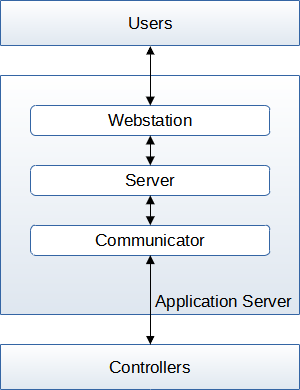
\includegraphics[width=0.3\textwidth]{images/scada_architecture.png}
    \caption{Arquitectura general de Rapid SCADA \cite{rapidscada_architecture}}
    \label{fig:scada_architecture}
\end{figure}

\subsection{Descripció dels components}

\subsubsection{Webstation}


És l'aplicació web encarregada de la visualització de dades i la interacció amb l'usuari. Permet accedir al sistema SCADA mitjançant un navegador web sense necessitat d'instal·lar programari addicional

Permet representar informació en forma de taules, gràfics o sinòptics, així com consultar dades històriques i enviar comandes. L'accés està controlat mitjançant usuaris i permisos definits per l'administrador i existeix la possibilitat d'ampliar aquesta aplicació mitjançant plugins per adaptar-se a diferents necessitats de visualització \cite{rapidscada_applications}.


\subsubsection{Communicator}

És el component responsable de la comunicació amb els dispositius de camp, com PLCs, sensors i controladors industrials.

La seva funció principal és adquirir dades en temps real i enviar comandes, gestionant múltiples línies de comunicació i diferents protocols industrials. Funciona en segon pla i registra l'activitat en fitxers de log per facilitar el diagnòstic d'errors \cite{rapidscada_applications}.

\subsubsection{Server}

Aquest component és el nucli del sistema Rapid SCADA. S'encarrega de gestionar l'emmagatzematge de dades, el processament i la distribució de la informació a la resta d'aplicacions.

Gestiona tant les dades en temps real com les històriques, controla l'accés dels usuaris i proporciona la informació a la resta de components. Funciona com un servei en execució contínua, sense interfície d'usuari. La seva configuració es realitza des de l'aplicació Administrator. La seva funcionalitat es pot ampliar mitjançant mòduls addicionals \cite{rapidscada_applications}.


\subsubsection{Agent}

Per un costat, \textit{Agent} és un servei encarregat de la gestió remota i la comunicació entre una instància de Rapid SCADA i l'aplicació Administrator.

Facilita la transferència de configuracions i l'accés als registres del sistema, permetent treballar tant en local com de forma remota mitjançant connexió TCP (port 10002 per defecte) \cite{rapidscada_applications}. Aquest component no disposa d'interfície gràfica i el seu funcionament es verifica mitjançant els registres del sistema.

\subsubsection{Administrator}

Per l'altre, \textit{Administrator} és l'eina principal de desenvolupament i configuració de Rapid SCADA. Actua com un entorn integrat que permet definir tota l'estructura del sistema.

Facilita la transferència de configuracions i l'accés als registres del sistema, permetent treballar tant en local com de forma remota mitjançant connexió TCP \cite{rapidscada_applications}.


També incorpora eines que faciliten el desenvolupament:
\begin{itemize}
    \item Assistents (wizards) per crear dispositius i canals
    \item Importació i exportació de configuracions
    \item Clonació de canals
    \item Funcions de cerca, filtratge i ordenació
\end{itemize}



\subsection{Gestió dels serveis}

Els components principals de Rapid SCADA funcionen com a serveis del sistema operatiu, iniciant-se automàticament per garantir la disponibilitat contínua del sistema.

En entorns Linux, aquests serveis es gestionen mitjançant eines com \texttt{systemctl}, mentre que en Windows es poden administrar des de les eines pròpies del sistema o des de l'Administrator \cite{rapidscada_services}.



\section{Configuració amb ScadaAdmin}

La configuració del sistema SCADA s'ha realitzat mitjançant l'eina \textit{ScadaAdmin}, que actua com a entorn principal de desenvolupament. \cite{rapidscada_config_basics}Aquesta permet crear i desplegar projectes que defineixen completament el sistema mitjançant fitxers, principalment en format XML.

\subsection{Estructura del projecte}

Un projecte de Rapid SCADA es divideix en diferents blocs principals:

\begin{itemize}
    \item \textbf{Configuration Database}: defineix l'estructura del sistema (objectes, dispositius, canals, usuaris)
    \item \textbf{Views}: conté les visualitzacions
    \item \textbf{Server, Communicator i Webstation}: configuració dels serveis del sistema
\end{itemize}

\subsection{Mòdul Database}

La base de dades de configuració és el nucli del sistema. Durant el desenvolupament es treballa en XML, però en el desplegament es transforma a format binari \texttt{.dat} optimitzat \cite{rapidscada_database}.


\subsubsection{Primary Tables}

Les \textbf{taules primàries} defineixen el funcionament principal del sistema. Són les més importants i s'han de configurar amb cura.

\begin{itemize}
    \item \textbf{Objects}: estructura jeràrquica del sistema (planta, línies, màquines)
    \item \textbf{Communication Lines}: defineixen les línies de comunicació amb els dispositius
    \item \textbf{Devices}: llista de dispositius físics o virtuals
    \item \textbf{Channels}: canals de dades (variables del sistema, sensors, actuadors)
    \item \textbf{Limits}: límits de valors (alarmes)
    \item \textbf{Views}: configuració de les visualitzacions
    \item \textbf{Roles i Users}: gestió d'usuaris i permisos
\end{itemize}

Aquestes taules estan interrelacionades. Per exemple, un dispositiu està associat a una línia de comunicació, i un canal està associat a un dispositiu.

\subsubsection{Secondary Tables}

Les \textbf{taules secundàries} complementen la configuració del sistema amb informació auxiliar.

\begin{itemize}
    \item \textbf{Archive kinds i Archives}: tipus i configuració d'arxius històrics
    \item \textbf{Channel types i Data types}: tipus de dades
    \item \textbf{Device types}: tipus de dispositius (drivers)
    \item \textbf{Formats}: formats de visualització
    \item \textbf{Units}: unitats de mesura
    \item \textbf{Scripts}: càlculs i fórmules
\end{itemize}

La Figura següent mostra l'estructura interna del projecte dins de ScadaAdmin:

\subsection{Procés de configuració}

 El procés recomanat de configuració és el següent \cite{rapidscada_config_basics}:

\begin{enumerate}
    \item Crear un nou projecte
    \item Definir objectes, línies de comunicació i dispositius
    \item Configurar el Communicator i la comunicació amb els dispositius
    \item Crear canals per gestionar les dades
    \item Definir visualitzacions (Views)
    \item Desplegar el projecte al servidor
\end{enumerate}

Aquest procés s'ha seguit en el desenvolupament del present TFG, adaptant-lo a la simulació de la planta industrial implementada en Unity.

\section{Visualització i interfícies}
La visualització es basa en el concepte de \textbf{Views} \cite{rapidscada_views}, que permeten representar i interactuar amb les dades del sistema a través de la Webstation \cite{rapidscada_views}.


\subsection{Tipus de vistes (\textit{Views})}

Rapid SCADA inclou per defecte diversos tipus de vistes, tot i que el sistema és extensible mitjançant plugins.


Cada vista es correspon amb un fitxer dins del directori \textit{Views} del projecte. Els tipus principals de vistes són:


\begin{itemize}
    \item \textbf{Table View} → fitxers de visualització tabular
    \item \textbf{Mimic Diagram} → esquemes gràfics del procés (plugin)
    \item \textbf{SchemClassic} → esquemes clàssics 
    \item \textbf{Faceplate} → components reutilitzables (plugin)
    \item \textbf{XML File} → configuracions personalitzades
    \item \textbf{Text File} → suport per definicions manuals
\end{itemize}

El sistema és extensible mitjançant plugins (mimics avançats, faceplates, etc.).

\subsubsection{Execució de les vistes}

Les vistes es mostren a través de la \textbf{Webstation}, que és l'aplicació web de Rapid SCADA accessible des d'un navegador.

El procés de visualització és el següent:

\begin{enumerate}
    \item Configuració a ScadaAdmin
    \item Registre a la taula Views
    \item Desplegament del projecte
    \item Accés des de Webstation segons permisos
\end{enumerate}

Les vistes poden incloure paràmetres com objecte associat, ordre o configuració específica (Figura \ref{fig:rapidscada_views}).

En el cas de les \textbf{Table Views}, aquestes permeten visualitzar dades històriques i en temps real. A més a més, es poden generar gràfiques clicant sobre els valors, permeten enviar comandes als dispositius i  utilitzen arxius històrics (Min, Hour, etc.) com a font de dades

La funcionalitat de les vistes es pot ampliar mitjançant plugins, que permeten crear interfícies més avançades i adaptades a les necessitats del sistema, com es detallarà en apartats posteriors.



\begin{figure}[H]
    \centering
    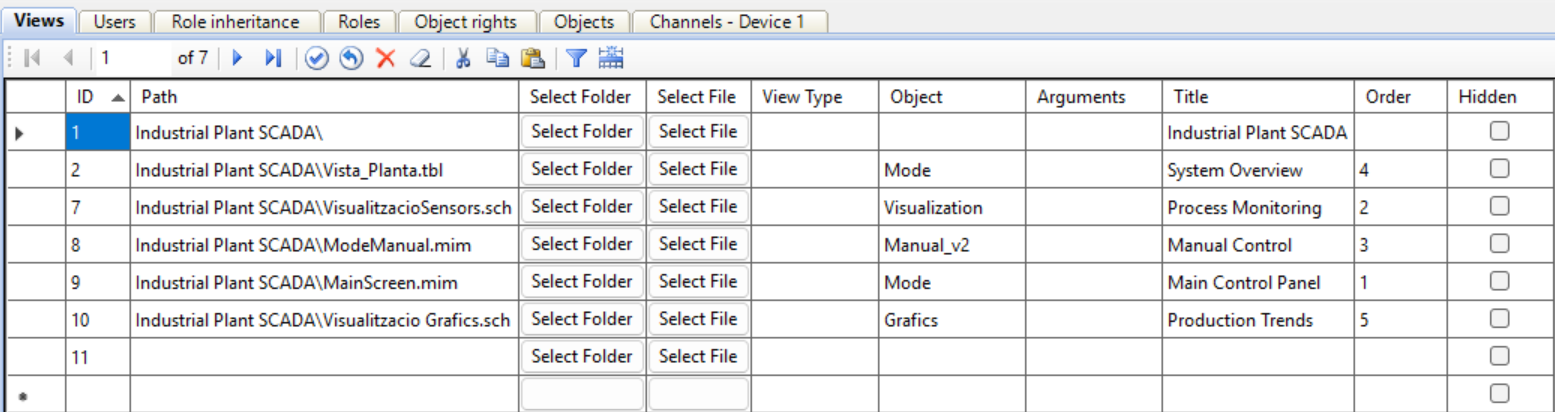
\includegraphics[width=0.6\textwidth]{images/views_scada.png}
    \caption{Taula \textit{Views} de RapidScada}
    \label{fig:rapidscada_views}
\end{figure}

\section{Comunicacions i dispositius}

La comunicació amb dispositius es gestiona mitjançant el mòdul \textbf{Communicator} i es basa en tres elements: \textbf{Communication Lines}, \textbf{Devices} i \textbf{Channels} \cite{rapidscada_device_polling, rapidscada_channels}. Aquests elements estan relacionats jeràrquicament: una línia de comunicació conté diversos dispositius, i cada dispositiu està associat a múltiples canals de dades. La configuració s'ha de realitzar seguint una seqüència lògica per garantir la coherència del sistema (Figura \ref{fig:rapidscada_comm}).

\subsection{Communication Lines}

Els canals de comunicació defineixen el mètode de connexió i permeten gestionar diverses connexions simultàniament.
Entre els principals tipus de canals suportats es troben: \textit{Port sèrie}, \textit{TCP Client}, \textit{TCP Server}, \textit{UDP} i \textit{MQTT Client}.


\begin{figure}[H]
    \centering
    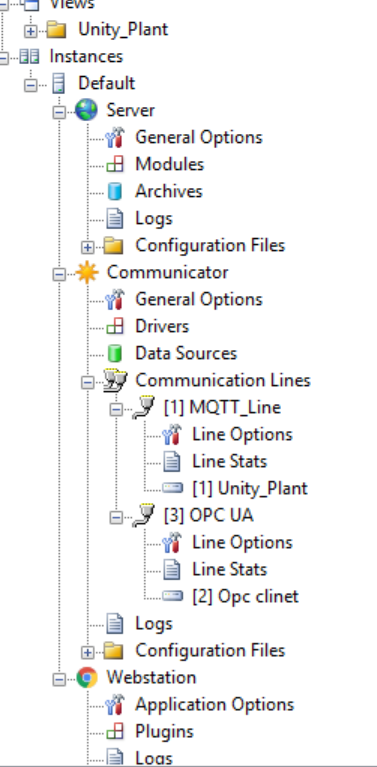
\includegraphics[width=0.3\textwidth]{images/communication.png}
    \caption{Vista general de les instàncies de RapidScada}
    \label{fig:rapidscada_comm}
\end{figure}

\subsection{Devices i polling}


Els \textbf{Devices} representen els dispositius físics o fonts de dades del sistema (PLC, sensors, actuadors o simuladors). \cite{rapidscada_device_polling} Cada dispositiu s'assigna a una \textit{Communication Line}, que defineix el canal de comunicació general, però la configuració específica del protocol es realitza principalment en el dispositiu mitjançant el \textbf{driver} seleccionat.

És a dir, la \textit{Communication Line} estableix el tipus de connexió (TCP, sèrie, MQTT, etc.), mentre que el \textit{Device} defineix com es comunica realment amb aquell equip. En alguns casos, com amb OPC UA o MQTT, la configuració pot dependre gairebé exclusivament del dispositiu.

En crear un dispositiu, es defineix el seu \textbf{device type} (driver), i posteriorment es poden ajustar els paràmetres principals dins de les opcions del dispositiu:


\begin{itemize}
    \item Driver (protocol de comunicació) i adreça (del dispositiu real amb el que vols comunicar-te.)
    \item Timeout i Delay
    \item Estat d'activació
\end{itemize}

El \textbf{polling} determina com es llegeixen les dades (cíclic, periòdic o sota demanda).

\subsection{Channels}

Els canasl són les unitats bàsiques de dades dins del SCADA (equivalents a variables o tags). Cada canal està associat a un dispositiu i a una variable concreta (sensor, estat, actuador, ...).

Les propietats més rellevants són:

\begin{itemize}
    \item \textbf{Data type}: tipus de dada (numèrica, booleana, etc.)
    \item \textbf{Tag}: identificador vinculat amb el dispositiu
    \item \textbf{Format}: representació visual
    \item \textbf{Limits}: definició d'alarmes
    \item \textbf{Archives}: on es guarden les dades (Min, Hour, etc.)
\end{itemize}

Els canals permeten emmagatzemar dades històriques, generar esdeveniments i enviar comandes als dispositius

\section{Gestió d'usuaris i permisos}

\subsection{Model de control d'accés}

Rapid SCADA utilitza un model de control d'accés basat en tres elements principals: \textbf{objectes}, \textbf{rols} i \textbf{usuaris} \cite{rapidscada_user_management}.

En primer lloc, es defineixen els \textbf{objectes}, que representen les diferents parts del sistema (planta, dispositius, zones o funcionalitats). Aquests objectes es poden organitzar de forma jeràrquica, permetent estructurar el sistema de manera lògica.

A continuació, es creen els \textbf{rols}, que defineixen un conjunt de permisos. A cada rol se li assignen drets específics sobre cada objecte, com ara visualització de dades o enviament de comandes.

Finalment, els \textbf{usuaris} es vinculen a un rol determinat. D'aquesta manera, cada usuari hereta automàticament els permisos associats al rol assignat.

Aquest model permet una gestió flexible i escalable dels accessos dins del sistema.

\subsection{Creació d'usuaris i assignació de rols}

Els usuaris es defineixen a la taula \textit{Users} i s'associen a un rol.

Alguns usuaris i rols bàsics es creen per defecte, com ara:
\begin{itemize}
    \item \textbf{Administrator}: accés complet
    \item \textbf{Dispatcher}: visualització i control
    \item \textbf{Guest}: només visualització
\end{itemize}

També es poden crear rols personalitzats amb permisos configurables, simplificant la gestió en sistemes complexos.


\subsection{Permisos i control d'accés}

Els permisos es defineixen a la taula \textit{Object rights}, indicant què pot fer cada rol sobre cada objecte.

Aquest sistema permet controlar accions com:
\begin{itemize}
    \item Visualitzar dades
    \item Accedir a pantalles
    \item Enviar comandes
\end{itemize}

Només els rols personalitzats poden tenir permisos configurables, ja que els rols predefinits ja tenen els seus drets definits internament. Per saber els permisos que tenen cada rol , es pot observar aquesta informació a la \textit{Rights Matrix} (Figura \ref{fig:rights_matrix})

\begin{figure}[H]
    \centering
    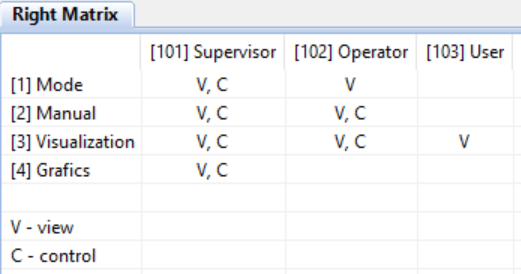
\includegraphics[width=0.5\textwidth]{images/right_matrix.png}
    \caption{Exemple de Rights Matrix a Rapid SCADA}
    \label{fig:rights_matrix}

\end{figure}

\subsection{Herència de permisos}

Rapid SCADA permet definir \textbf{herència de rols}, de manera que un rol pot heretar els permisos d'ltres rols. Això permet reutilitzar configuracions i reduir la complexitat.

A més, com que els objectes poden estar organitzats jeràrquicament, els permisos assignats a un objecte superior es propaguen als seus subobjectes, facilitant la gestió en sistemes grans.

\section{Gestió de dades i bases de dades}

Rapid SCADA disposa de diferents mecanismes per a l'emmagatzematge de dades, combinant un sistema intern optimitzat amb la possibilitat d'integració amb bases de dades externes.

\subsection{Emmagatzematge intern}

Per defecte, Rapid SCADA no utilitza una base de dades relacional clàssica per al funcionament en temps real. En lloc d'això, el sistema emmagatzema les dades en fitxers binaris amb extensió \texttt{.dat}, situats principalment a la carpeta \textit{Archive}.

Aquests fitxers estan optimitzats per a:
\begin{itemize}
    \item Accés ràpid a dades temporals
    \item Emmagatzematge eficient de grans volums d'informació
    \item Funcionament continu en sistemes industrials (24/7)
\end{itemize}

És important destacar que aquest format \textbf{no permet la realització de consultes SQL directes}. L'accés a les dades es realitza exclusivament a través dels mòduls interns del sistema, com la Webstation (taules, gràfics) o mitjançant plugins específics d'exportació.

\subsection{Bases de dades externes}

El sistema permet integrar bases de dades externes com \cite{rapidscada_overview}:

\begin{itemize}
    \item \textbf{PostgreSQL}: base de dades relacional per a emmagatzematge estructurat
    \item \textbf{InfluxDB}: base de dades orientada a sèries temporals, especialment adequada per dades SCADA
\end{itemize}

Aquesta integració permet:
\begin{itemize}
    \item Emmagatzemar dades en formats consultables mitjançant SQL 
    \item Realitzar anàlisi avançada de dades
    \item Integrar el sistema amb altres aplicacions externes
\end{itemize}

En aquests casos, \cite{rapidscada_db_export} les dades es transfereixen des del sistema intern de Rapid SCADA cap a la base de dades externa, on sí que es poden executar consultes, informes i processos analítics.

\section{Plugins de Rapid SCADA}

\subsection{Consideracions generals sobre plugins}

Rapid SCADA permet ampliar les seves funcionalitats mitjançant \textbf{plugins} i mòduls addicionals. En el cas de la Webstation, aquests mòduls s'anomenen plugins i permeten estendre la interfície d'usuari i les capacitats de visualització.

Mitjançant plugins es poden implementar:
\begin{itemize}
    \item Nous tipus de vistes
    \item Components gràfics per a esquemes
    \item Gràfiques i informes avançats
\end{itemize}

Es desenvolupen en \textit{.NET} \cite{developers} i s'integren com a llibreries \texttt{.dll}. També es poden obtenir des del repositori oficial o des de la botiga de mòduls de Rapid SCADA.

\subsection{Sistema de llicències i instal·lació}

Els plugins poden tenir diferents modalitats:
\begin{itemize}
    \item \textbf{Gratuïts}: inclosos per defecte o disponibles públicament
    \item \textbf{De pagament}: requereixen registre i clau de llicència
    \item \textbf{Versió trial}: funcionament limitat sense registre, el qual ens obliga a demanar un codi que dura 24 hores cada vegada que volguem instal·lar aquests plugins. 
\end{itemize}

El procés d'instal·lació consisteix en:
\begin{itemize}
    \item Copiar els fitxers del plugin a la carpeta d'instal·lació de SCADA
    \item Activar-lo des de \textit{ScadaAdmin}.
    \item Configurar-lo segons la seva documentació
    \item Carregar el projecte al sistema
\end{itemize}


\subsection{Plugins utilitzats en el projecte}

\subsubsection{Chart Pro Plugin}

Aquest plugin \cite{rapidscada_chart_pro} amplia les capacitats de visualització de dades, permetent representar gràfiques avançades amb múltiples canals simultanis.

Les seves funcionalitats principals són:
\begin{itemize}
    \item Visualització de múltiples canals en un mateix gràfic
    \item Modes de visualització (fix o dinàmic)
    \item Exportació a formats com PNG o PDF
    \item Configuració mitjançant perfils
\end{itemize}

S'ha utilitzat per representar l'evolució temporal de variables del sistema, millorant la visualització respecte al sistema base (Figura \ref{fig:chart_pro}).


\begin{figure}[H]
    \centering
    \includegraphics[width=0.5\textwidth]{images/chart-pro-example.png}
    \caption{Exemple del modul ChartPro \cite{rapidscada_chart_pro}}
    \label{fig:chart_pro}
\end{figure}

\subsubsection{Extra Scheme Editor}

El sistema base de Rapid SCADA permet la creació d'esquemes mitjançant fitxers \texttt{.sch}, amb elements bàsics com textos, imatges, botons, indicadors (LED) i enllaços (Aplicació d'aquesta part en el apartat HMI\_RAPIDSCADA.TEX)
El \textbf{Extra Scheme Editor} amplia aquestes funcionalitats afegint nous components gràfics com \textbf{Chart} (gràfiques de dades), \textbf{Trend}, \textbf{Gauge} (indicadors analògics) o \textbf{Frame}

Especialment rellevant és l'ús del component \textbf{Chart}, que, combinat amb el Chart Pro Plugin, permet visualitzar múltiples canals en temps real dins dels esquemes.

Tot i això, cal destacar que les gràfiques integrades en fitxers \texttt{.sch} tenen funcionalitats més limitades en comparació amb les visualitzacions generades des de les vistes de tipus taula (\texttt{.tbl}). En aquestes últimes, en seleccionar una variable amb dades històriques, es poden generar gràfiques més completes, amb opcions avançades com la selecció de períodes de temps o la visualització detallada de l'evolució de les dades.

\subsubsection{Mimic Editor}

El \textbf{Mimic Editor} és un plugin que permet crear interfícies gràfiques més avançades i flexibles que els fitxers \texttt{.sch}.

A diferència dels esquemes tradicionals, aquest editor permet:
\begin{itemize}
    \item Associar comportaments dinàmics als elements gràfics 
    \item Definir accions en interaccions (clics) (no solament als botons o al \textit{toggle}).
    \item Enviar valors específics directament a canals (control actiu) sense limitació
\end{itemize}

A més, permet integrar els components del \textit{Extra Scheme Editor}, combinant visualització i control en una mateixa interfície.

Aquest plugin ha estat clau en el desenvolupament del projecte, ja que permet una interacció més completa amb el sistema SCADA i facilita la implementació del control sobre la planta simulada.


\end{document}
